%!TEX root = ../template.tex
%%%%%%%%%%%%%%%%%%%%%%%%%%%%%%%%%%%%%%%%%%%%%%%%%%%%%%%%%%%%%%%%%%%%
%% chapter5.tex
%% NOVA thesis document file
%%
%% Chapter with lots of dummy text
%%%%%%%%%%%%%%%%%%%%%%%%%%%%%%%%%%%%%%%%%%%%%%%%%%%%%%%%%%%%%%%%%%%%
\chapter{Evaluation}
\label{cha:evaluation}

%\textbf{TOPICS :}
%\begin{itemize}
%	\item Benchmark the iCBD-Replication Module
%	\item Assert the performance gained by storing iMI closer to client workstations
%\end{itemize}

This chapter reports the experimental work performed in order to study both the functionality and performance of the Replication and Caching Service. We start by laying out the test plan followed by the results that we collected. We then analyse those results, always trying to co-relate them with other events observed in the platform.

The chapter is divided into the following sections:

\begin{description}
    %
    \item [Section~\ref{sec:eval_exp_setup}] begins by showing how it was applied and what changes were needed to the infrastructure described in the previous chapter, in order to carry out all the measurements that we propose to evaluate.
    %
    \item [Section~\ref{sec:eval_method}] overviews the two procedures applied for the evaluation of the Replication and Caching Service, both for functional validation and performance analysis.
    %
    \item [Section~\ref{sec:eval_rep_bench}] shows how was developed the benchmark for the performance test of the replication module, then presents the results of those tests, and ends with a comparative analysis.
    %
    \item [Section~\ref{sub:eval_cache_bench}] finally details the performance tests conducted to the inclusion of a cache server in the iCBD platform, taking into account the boot time of the workstations and the provenience of the iMIs.
    %
\end{description}

\newpage

%%-------------------------------------------------------------------
%%	5. - Motivation
%%-------------------------------------------------------------------
%\section{Motivation}
%\label{sec:eval_motivation}

%https://stackoverflow.com/questions/1198691/testing-io-performance-in-linux
%https://dl.acm.org/citation.cfm?id=1367829.1367831

%https://github.com/axboe/fio
%https://github.com/giantswarm/filesystem-benchmark


%%-------------------------------------------------------------------
%%	5. - Experimental Setup
%%-------------------------------------------------------------------
\section{Experimental Setup}
\label{sec:eval_exp_setup}

As discussed in the previous chapter, the DI (Computer Science Department) provided two laboratories (Lab 110 and Lab. 112) fully equipped with fifteen desktop PCs each (the general specifications of those machines can be seen in the table~\ref{tab:exp_lab_work}), for the validation of the caching solution both at the functional and performance levels.

\begin{table}[]
\centering
\begin{tabular}{ll}
\textbf{CPU} & Intel Core i3-7100 @ 3.90GHz \\
\textbf{Memory} & 8 GB \\
\textbf{Storage} & 275GB SSD \\
\textbf{Ethernet} & 1 Gbps
\end{tabular}
\caption{Specifications of the Laboratories Workstations}
\label{tab:exp_lab_work}
\end{table}


To ensure the correct execution of all the tests we had planned, some adjustments to the iCBD platform were necessary. From the infrastructure point-of-view, we deployed two more virtual cache servers (raising their number to a total of three).
From a functional point-of-view, the iCBD-rw and iCBD-home VMs were moved to the same networks (VLANs) of these labs, and their interfaces configured with the appropriate static IPs. Then, a vNIC (Virtual Network Interface Card) of the iCBD-imgs VM was connected to the Lab. 110 VLAN and assigned the appropriate fixed IP. This restructuring also required changes in the iCBD configuration files to allow the lab’s workstations to access iMIs. The Physical Cache Server also had one of its NICs configured in the Lab. 112 VLAN, and similar configurations were necessary in order to allow the server to provide iMIs to the lab’s workstations.

\begin{table}[htpb]
\centering
\begin{tabular}{lcc}
%\hline
                             & \textbf{FCT NOVA}          & \textbf{SolidNetworks (Development)}              \\ \hline
\textit{\textbf{Servers}}    & 2x HPE ProLiant DL380 Gen9 & 2 x HPE ProLiant DL380 Gen9   \\
\textit{\textbf{Switch}}     & HPE Flexfabric 5700 jg898a & HPE Flexfabric 5700 jg898a    \\
\textit{\textbf{Disk Array}} & HPE MSA 2040 SAN Storage   & N/A - (Storage on the Server) \\
\textit{\textbf{Networking}} & 10 Gbps (between servers)  & 10 Gbps (between servers)     \\ \hline
\end{tabular}
\caption{Physical infrastructure of the FCT NOVA and SolidNetworks sites}
\end{table}

Finally, two more (but important) aspects should be referred: first, the Physical Cache Server and the Lab. 112 workstations were attached to the same switch, so the traffic flowing between them was internal to the device, whereas all communications between workstations (of the two labs) and the iCBD VMs had to cross a few switches in the faculty’s network and therefore may suffer from adverse network conditions that were entirely out of our control; the second aspect is link speeds - all connections are 1 Gbps links, including the physical interfaces of the servers and virtual interfaces of the VMs. A simplistic schematic of all connections can be found in Figure~\ref{fig:eval_setup}.

\begin{figure}[htbp]
	\centering
	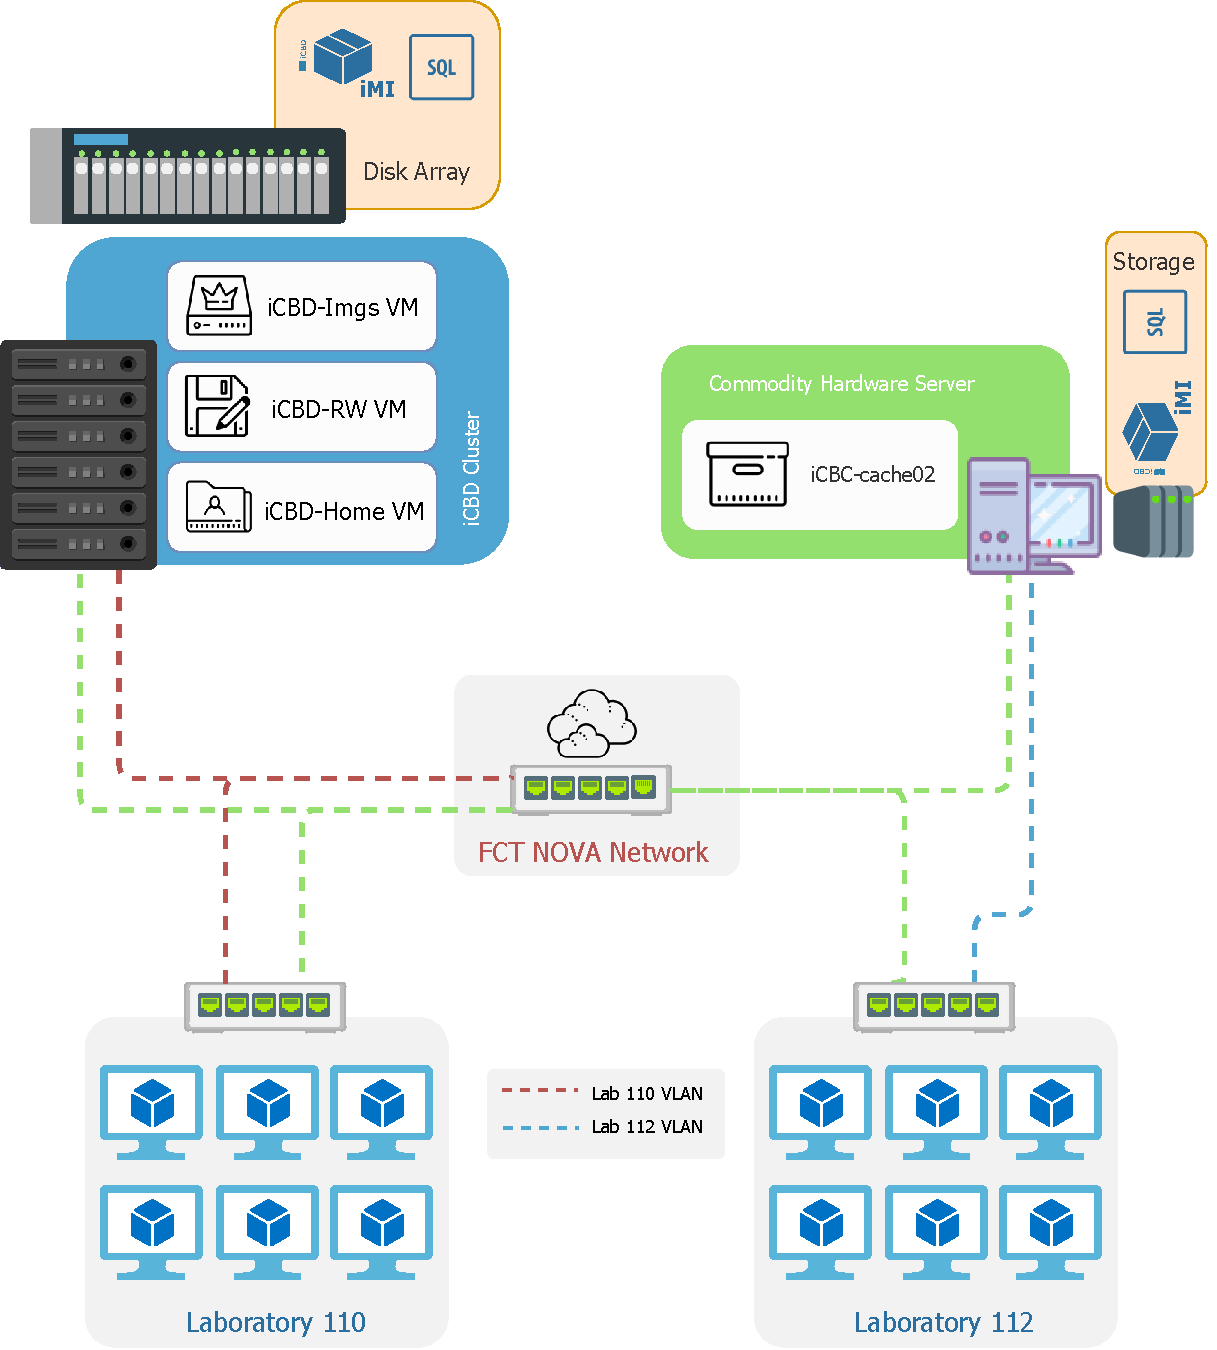
\includegraphics[height=4in]{cap5_lab_setup}
	\caption{iCBD Nodes and Networking Setup}
	\label{fig:eval_setup}
\end{figure}




%%-------------------------------------------------------------------
%%	5. - Metodology
%%-------------------------------------------------------------------
\section{Metodology}
\label{sec:eval_method}

The analysis of the RCS was performed in two distinct moments: in the first moment, we addressed the functional validation of RCS (we covered both components, replication and caching), after being integrated into the iCBD platform - the tests were to assert its correct operation; in the second moment, our focus was on the performance of both components in a production environment.

\paragraph{Functional validation}
\label{par:eval_func_val}

In order to test the functional correctness of the replication module in a multi-node environment, the Master Node was started in the iCBD-imgs VM and three Replica Nodes were also started, one in each Cache Server (virtual: iCBD-cache01 and iCBD-cache03; physical - iCBD-cache02). We observed that the Replica Nodes had registered themselves on the Name Server, as expected, and that the communications between the Master Node and Replicas also performed as expected.
Next, were repeatedly carried out two types of tests: one focused on sending a full iMI version (one that was not present in the Replicas’ Image Repository), forcing the data to be copied over the network.
Furthermore, we wanted to verify that, when the transfer completed, the local Image Repository reflected the addition of the new iMI. This scenario is likely to occur the first time that a replica subscribes to a new iMI.

The second type of test addressed the process of sending iMI versions that were newer than those already available at Replica nodes. This test simulates the case where, after the administration of an iMI, the new, updated version should be distributed to the Replicas with conservation of bandwidth, i.e., where only the data differences were transferred. At the end of each test, a calculation of an MD5 hash was performed with the \texttt{md5sum} tool, in order to ensure that the received data was being reliably transferred and the replica was identical to the original.

Functional testing of Cache Servers was performed with iCBD-cache02, the physical Cache Server, mostly because it was connected directly to one of the labs and thus allowing for immediate testing of a workstation’s iMI boot. Given the degree of integration of the iCBD platform with the remaining network services and policies of FCT NOVA, a considerable iterative process of experimentation was required, tuning some parameters of a few iCBD services until we arrived at a fully functional configuration. In the end, it was confirmed that it was indeed possible to boot the workstations with iMIs delivered by the Cache Server.

\paragraph{Performance Benchmarking}
\label{par:eval_perf_bench}

In this second phase of our tests, the goal was to ascertain the performance of RCS in a production environment. In the case of the replication module, we compared the results obtained from multiple configurations of our implementation (transfers performed with or without compression and over secure or plain communication channels) and the \texttt{rsync} tool; we measured both the time spent on the transfer as well the amount of data transmitted between nodes.

Another important metric that we observed was the time spent on the boot process of a workstation, and we compared the results obtained in the case where the iMI was transferred from the Cache Server against those gathered when it was transferred by the iCBD-imgs VM hosted at the cluster (this one was provided with more resources – vCPUs and vRAM). The time spent on the boot process was computed as the elapsed time between the start of the kernel loading operation, to the moment when the initialisation of all user-space services was finished. The utility that gathered these events was \texttt{systemd-analyze}.

Finally, unless otherwise stated, all tests were executed five times; the best and worst results were then removed, and the final result is the average of the remaining values. The results of the benchmark are laid out in the following sections.


%%-------------------------------------------------------------------
%%	5. - Replication Service Benchmark
%%-------------------------------------------------------------------
\section{Replication Service Benchmark}
\label{sec:eval_rep_bench}

Let’s just briefly recall the two tests that we set out to perform: one, focused on sending a full iMI version (one that was not present in the Replicas’ Image Repository), forcing the data to be copied over the network; the other focused on sending iMI versions that were newer than those already available at Replica nodes, which should receive only receive the differences (deltas) associated with the new version.

For these tests, a Linux iMI containing an Ubuntu Desktop 16.04 LTS distribution (with quite a few “extras”, such as OpenOffice) was chosen, and two consecutive versions, v1 and v2 were used. These versions were created as follows: v1, the base version of this iMI, occupies 38.60GB; we started an administration VM and performed a full update with the \texttt{apt} tool (an \texttt{apt-get update} followed by an \texttt{apt-get upgrade}), and committed the results to the new version, v2.

Using the \texttt{btrf-progs} package we issued the command \texttt{btrfs filesystem df /path/} to retrieve Btrfs’ view about the differences between versions v1 and v2, which the utility reported as being 4.45 GB.


For both test scenarios, we created four different settings for the transfer tests:

\begin{description}
	%
	\item [Rsync] Transfer of an iMI using the rsync tool \footnote{It should be noted that the rsync tool is not aware of a Btrfs subvolume, so the times presented only relate to data transmission, but more operations would be needed to make the iMI functional within the iCBD platform.} with the options \texttt{-r} (recurse into directories); \texttt{-t} (preserve modification times); \texttt{-p} (preserve permissions); \texttt{-l} (copy symlinks as symlinks) and \texttt{-u} (skip files that are newer on the receiver).
	%
	\item [iCBD-Rep - I] Use the iCBD-Replication platform services to transfer the iMI using the standard Python sockets, and no compression.
	%
	\item [iCBD-Rep - II] Use the iCBD-Replication platform services to transfer the iMI using the standard Python sockets , with compression using the LZ4 algorithm over the data stream.
	%
	\item [iCBD-Rep - III] Use the iCBD-Replication platform services to transfer the iMI over an SSH tunnel, without compression.
	%
\end{description}

%\subsubsection{Sending a complete version of an iMI}
%\label{susub:eval_iMI_full}

\paragraph{Sending a complete version of an iMI}
\label{par:eval_iMI_full}

This test that sends a complete iMI, that is, all its 38.60GB of data; we observed that our iCBD replication module performs similarly on the three tests (I to III), but lags when compared to rsync; the results are shown in Table~\ref{tab:eval_imifull}.
It also shows that the rsync transfer process is faster than our Python-plus-btrfs-send code; however, using rsync has a drawback: after the transfer is complete, we have to use the Btrfs tools to recreate the versioning structure, and that takes time (which we have not measured).

\begin{table}[h]
\centering
\begin{tabular}{lcc}
 & \textbf{Time} & \textbf{Data Sent (MB)} \\ \cline{2-3} 
\textit{\textbf{Rsync}} & 12m23s & 39543 \\
\textit{\textbf{iCBD-Rep - I}} & 17m21s & 38947 \\
\textit{\textbf{iCBD-Rep - II}} & 20m35s & 35572 \\
\textit{\textbf{iCBD-Rep - III}} & 22m55s & 39412
\end{tabular}
\caption{Time spent and data transmitted on transferring a complete iMI from Master to Replica}
\label{tab:eval_imifull}
\end{table}

The tests also indicate that the IMI is compressible, with savings at around 8.6\%. Compression, when applied to a btrfs-send stream, is applied to both data and instructions generated by the send operation.


%\subsubsection{Sending only the delta between version of an iMI}
%\label{susub:eval_iMI_delta}

\paragraph{Sending only the delta between version of an iMI}
\label{par:eval_iMI_delta}

We now present the results for the test cases where just the differences between the two versions of the iMI were transferred. From the outset, one can see, as expected, a drastic reduction on the amount of data transmitted over the network. The results are shown in Table~\ref{tab:eval_imidelta}.

\begin{table}[h]
\centering
\begin{tabular}{lcc}
 & \textbf{Time} & \textbf{Data Sent (MB)} \\ \cline{2-3} 
\textit{\textbf{Rsync}} & 10m15s & 5964 \\
\textit{\textbf{iCBD-Rep - I}} & 1m47s & 4864 \\
\textit{\textbf{iCBD-Rep - II}} & 2m15s & 4713 \\
\textit{\textbf{iCBD-Rep - III}} & 2m55s & 4902
\end{tabular}
\caption{Time spent and data transmitted on transferring a delta between v1 and v2 of an iMI from Master to Replica}
\label{tab:eval_imidelta}
\end{table}

Our solution using Btrfs \texttt{send} and \texttt{receive} operations shows it to be far superior to rsync’s performance on the same data set. Even in the cases where the compression or cypher options were used, the results did not change dramatically. Here, our conclusion for the staggering difference between rsync and our solution(s) is that rsync takes an enormous amount of time computing the differences (with block-by-block comparisons) and “deciding” on what to send.

%This is an optimum taking into account that these two operations are computationally heavy and therefore in addition to placing more load on the machines that by themselves with the replication process already throw high load values

%\textbf{TOPICS :}
%\begin{itemize}
%	\item Replication with rsync (100 / 1000 mbps)
%	\item Replication with iCBD-Replication - Plain Sockets and No Compression (100 / 1000 mbps)
%	\item Replication with iCBD-Replication - Plain Sockets and LZ4 Compression (100 / 1000 mbps)
%	\item Replication with iCBD-Replication - Plain Sockets and zlib Compression (100 / 1000 mbps)
%	\item Replication with iCBD-Replication - Plain Sockets and snappy Compression (100 / 1000 mbps)
%	\item Replication with iCBD-Replication - SSH and No Compression (100 / 1000 mbps)
%\end{itemize}

%https://stackoverflow.com/questions/5357601/whats-the-difference-between-unit-tests-and-integration-tests

% Unit Test Python
%https://docs.python.org/2/library/unittest.html

%Memory profile of the module
%https://pypi.python.org/pypi/memory_profiler

%%-------------------------------------------------------------------
%%	5. - Cache Server Performance Benchmark
%%-------------------------------------------------------------------
\section{Cache Server Performance Benchmark}
\label{sub:eval_cache_bench}

With this next benchmark we present, we want to evaluate the behaviour of introducing a Cache Server in a production environment. In order to obtain some interesting metrics, two types of tests were carried out, one scenario in which five workstations are sequentially booted, and the second experiments with the extreme case in which all the machines in a laboratory are connected at the same time, creating a situation known as boot storm. For each scenario, we measured the boot times of each workstation, and with a tool called netdata~\cite{netdata} monitored the state of the server at the time it is serving the iMis.

In addition to the two scenarios, there are more variables in play. All tests were performed with all links connected at Gigabit speed. Then every single one was repeated with links limited to 100 Mbps. For this to happen, on the tests referring to the Cache Server, the interface that serves the Lab. 112 was configured at this slower speed. As for the VM that serves the Lab. 110, iCBD-imgs, the type of virtual interface employed does not allow the change of its speed but using the Traffic Shaping feature of the Distributed VSwitch, we managed to limit the bandwidth of the entire PortGroup that refers to this laboratory, in the end reaching the goal.

Lastly, we need to explain the three types of boot tested in this section. The iMI chosen for these tests was the same as mentioned above, a Linux iMI with the Ubuntu 16.04 LTS distribution.

\begin{description}
	%
	\item [Linux Server VDI] In this case, the computation is done on one of the cluster nodes in a diskless VM, simulating a traditional VDI environment, with the particularity of using the iCBD platform's network boot. This variant was born due to its versatility during the development of the platform, since we can connect this VM to any of the networks (internal or labs) and perform tests on its operation.
	%
	\item [Linux iCBD Native] When we talk about this variant, we are addressing the boot of an iMI in a physical workstation in which, in this case, the OS Linux runs natively on top of the hardware, with no kind of resource to virtualisation.
	%
	\item [Linux iCBD VM] This last variant presents an interesting feature since it makes use of two iMIs. In a first phase, it boots as described in the previous point, but with two differences. The booted iMI is of an openSUSE 42.2 \footnote{In this case, any other iMI could be used as a base (including natively run and then virtualised the same iMI), the version  42.2 of openSUSE was chosen because it was the iMI that exhibited the best stability in virtualising any other iMI, throughout the development process.}, and this iMI has installed the VMware Workstation Player serving as a foundation to the next one. When the openSUSE iMI boot process ends, the iMI Ubuntu 16.04 is loaded by VMware Player and is then run on a virtual machine. All this without the user realising that he is using a virtual machine running on a different OS.
		%
\end{description}

It is important to note that not only tests were performed with Linux iMIs, during the development of iMIs were tested with Windows 7 and Windows 10. It was decided not to include any of the tests performed with these iMIs because there was detected an unresolved issue that led the boot process to be abnormally slow. Something that was only found on the FCT NOVA site, since on the SolidNetworks site we did not detect any problems, and the Windows iMIs boot process is nominal.




\paragraph{Benchmark Sequential Boot}
\label{par:eval_cache_bootstorm}

\begin{table}[h]
\centering
\begin{tabular}{llcc}
\textbf{iMI} &  & \textbf{iCBD-imgs} & \textbf{iCBD-Cache02} \\ \hline
\multirow{2}{*}{\textit{Linux Server VDI}} & iSCSI & 453.5 MB & 454.3 MB \\
 & NFS & 703.0 MB & 702.1 MB \\ \hline
\multirow{2}{*}{\textit{Linux Client Native}} & iSCSI & 456.3 MB & 453.6 MB \\
 & NFS & 704.2 MB & 703.8 MB \\ \hline
\multirow{2}{*}{\textit{Linux Client VM}} & iSCSI & 834.1 MB & 836.8 MB \\
 & NFS & 950.5 MB & 952.8 MB
\end{tabular}
\caption{Total data received after booting, given each boot variant and for both iMI providers}
\label{tab:boot_totaldata}
\end{table}

In this case, we perform the boot tests of the workstations in varying two parameters - link speed (1 Gbps and 100 Mbps) and protocol used (iSCSI and NFS). It has been found that by changing the protocol by which workstations boot, the amount of data that is transferred from the repository (iCBD-imgs or iCBD-cache02) is influenced as shown in the Table~\ref{tab:boot_totaldata}. We can attribute this variation to the fact that the NFS protocol is a bit more resource hungry, resulting in the need to transfer a larger amount of data. This ultimately means that the workstations that boot using this protocol will also spend more time in this process. As can be observed when comparing Figures~\ref{fig:boot_iscsi} and ~\ref{fig:boot_nfs}.


\begin{figure}[htbp]
	\centering
	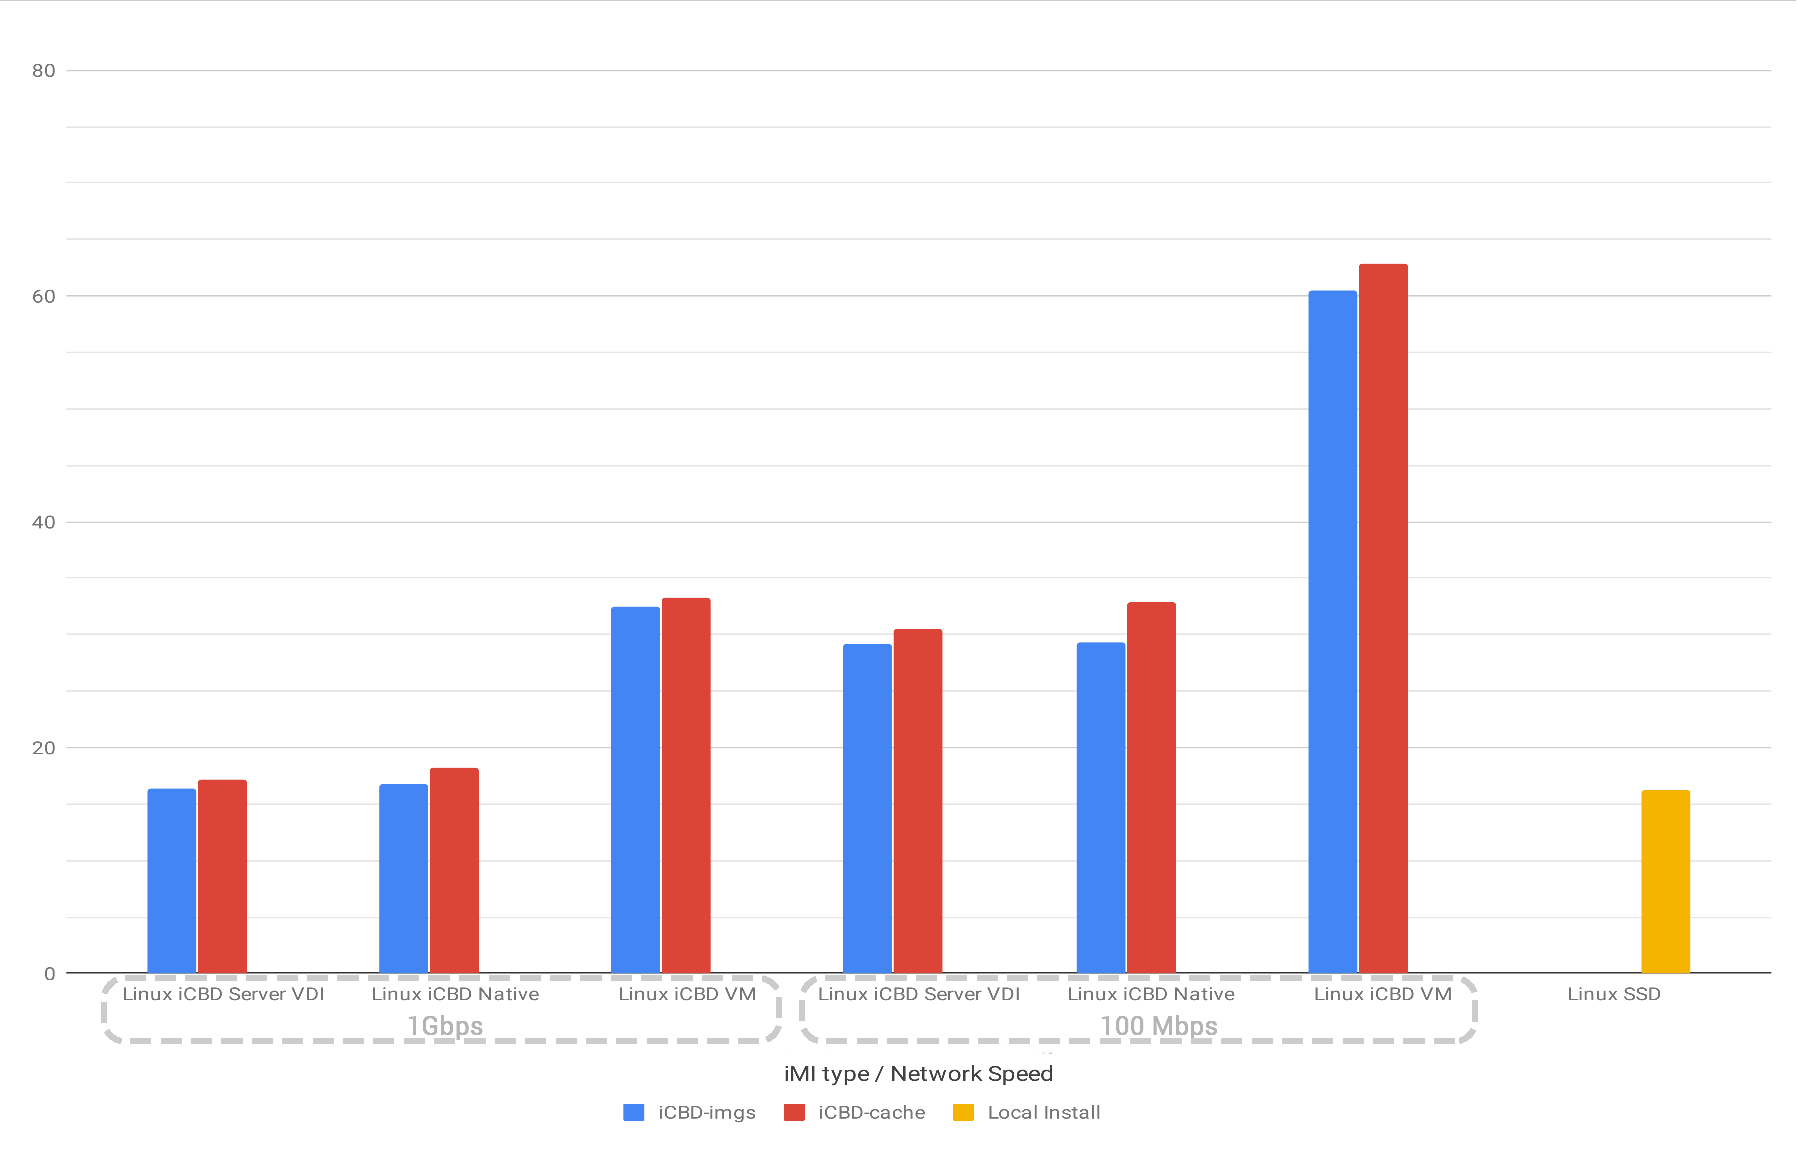
\includegraphics[height=4in]{cap5_NB_iSCSI}
	\caption{Mean Boot Time of five workstations using iSCSI (Sequential Boot Scenario), comparing iMI provider and network speed}
	\label{fig:boot_iscsi}
\end{figure}

\begin{figure}[htbp]
	\centering
	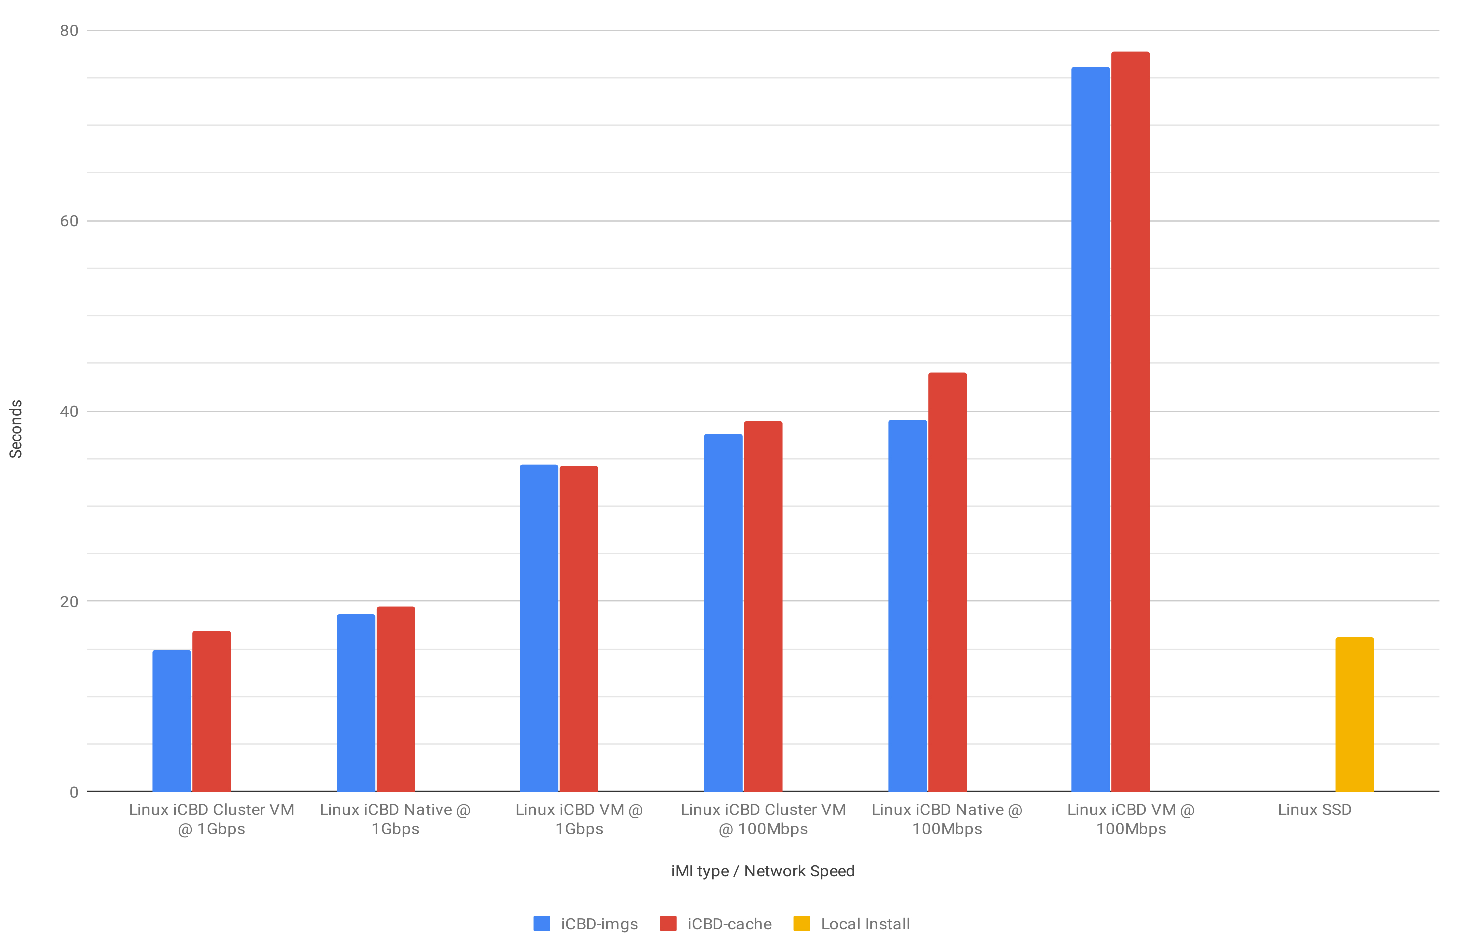
\includegraphics[height=4in]{cap5_NB_NFS}
	\caption{Mean Boot Time of five workstations using NFS (Sequential Boot Scenario), comparing iMI provider and network speed}
	\label{fig:boot_nfs}
\end{figure}


As for running tests varying the speed of the links, a significant degradation can be observed, with the workstations taking much longer in the boot process when the link speed was set at 100 Mbps.
Having the extreme case, when doing tests with the boot type Linux iCBD VM in which the average of the times passes the minute mark.
Finally, we can observe that workstations booting from the iCBD-cache02 spend more time in this process than the ones that boot from iCBD-imgs, although latency in the first case is theoretically lower. We can attribute these results to the fact that iCBD-cache02 has much lower specifications than iCBD-imgs. Which leads us to believe that the solution can be vertically scalable. Metrics regarding the behaviour of both servers during one of these tests can be observed in the Figures~\ref{fig:boot_imgs_stats} and ~\ref{fig:boot_cache_stats}.


\begin{figure}[htbp]
	\centering
	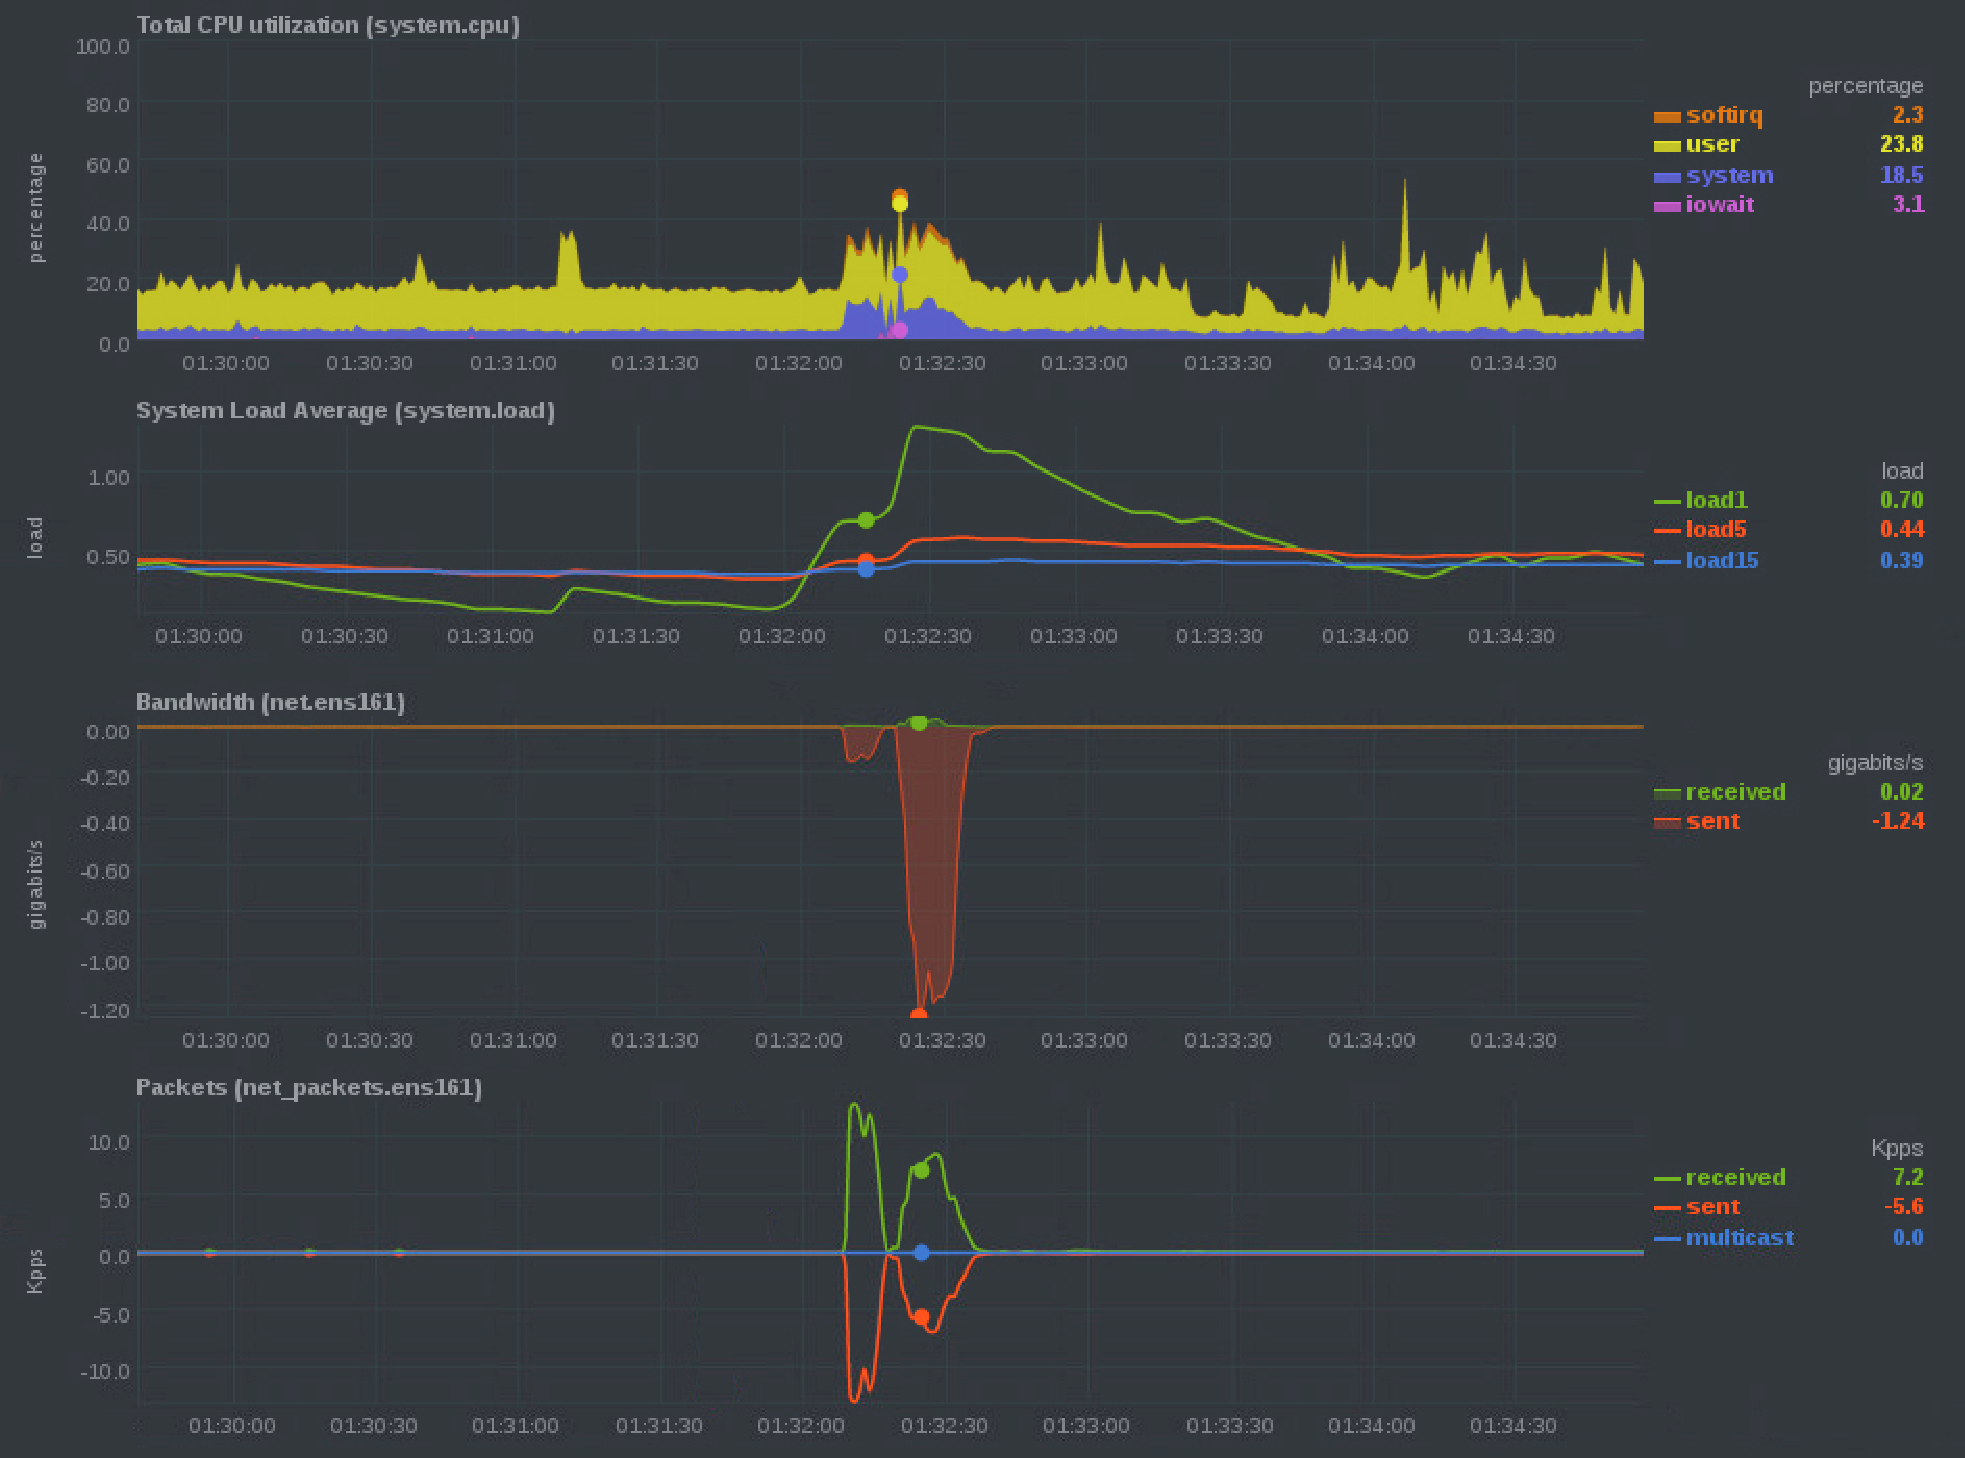
\includegraphics[height=4in]{cap5_secboot_imgs_stats}
	\caption{System metrics for iCBD-imgs on one run of the five workstations sequential boot scenario test}
	\label{fig:boot_imgs_stats}
\end{figure}


\begin{figure}[htbp]
	\centering
	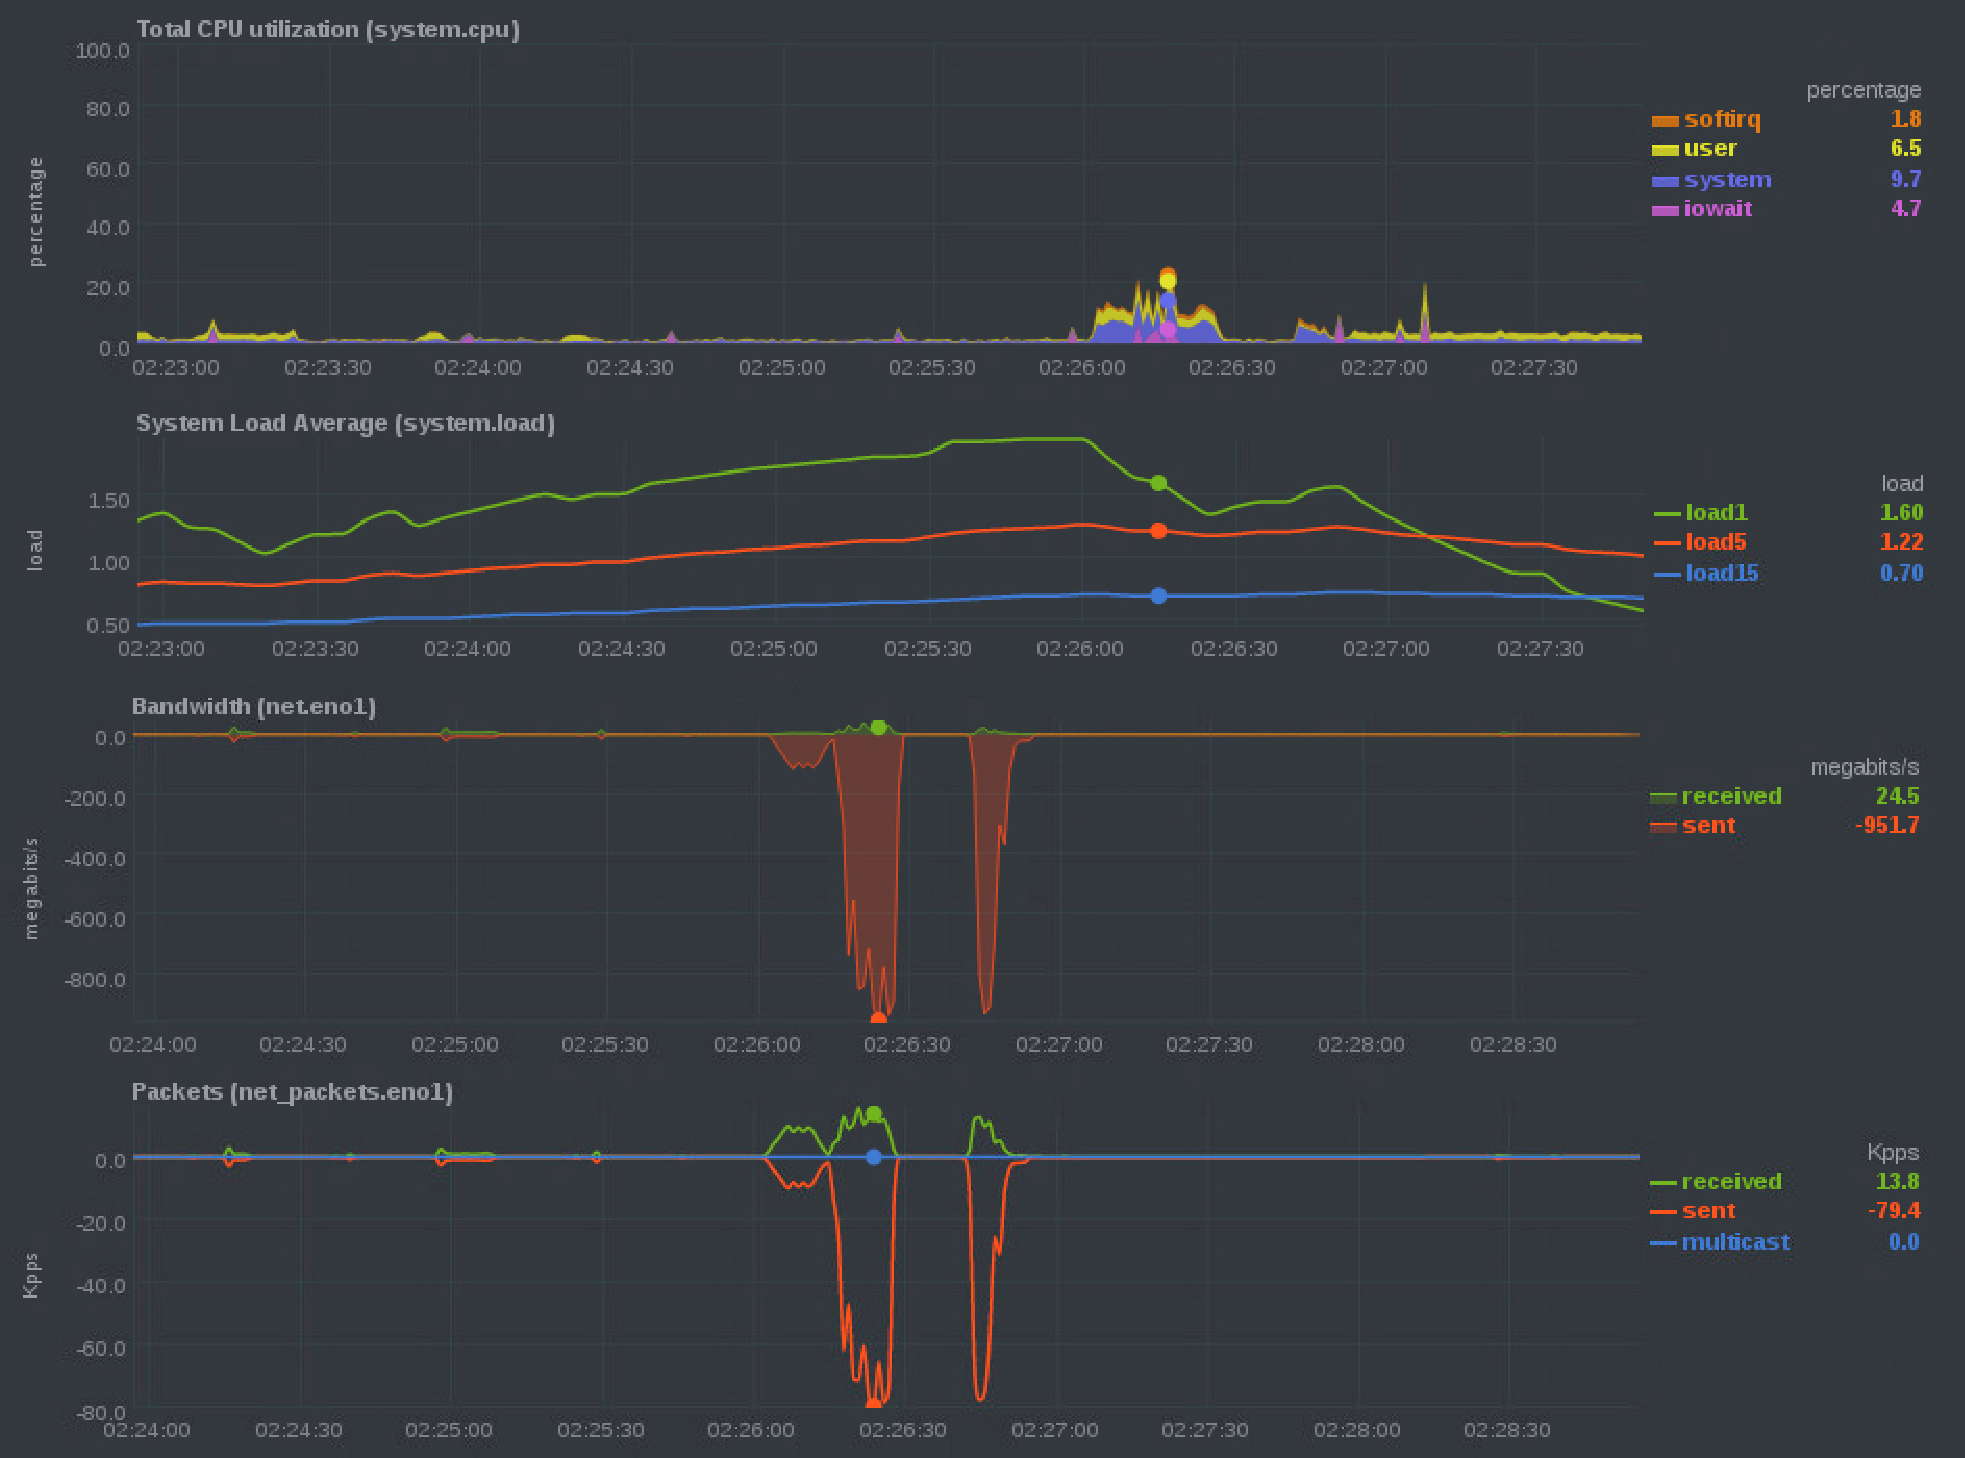
\includegraphics[height=4in]{cap5_secboot_cache_stats}
	\caption{System metrics for iCBD-Cache02 on one run of the five workstations sequential boot scenario test}
	\label{fig:boot_cache_stats}
\end{figure}


%\subsubsection{Benchmark in a Boot Storm condition}
%\label{susub:eval_cache_bootstorm}
\paragraph{Benchmark in a Boot Storm condition}
\label{par:eval_cache_bootstorm}


Finally we present the results of a test carried out in a boot storm scenario. Some simplifications have been made for this. First, no tests were performed using the Linux Server VDI boot type, so all values result from the measurement of boot time of the 15 workstations of both laboratories.

On the other hand, these tests were also performed only with the link speed of 1 Gbps\footnote{Although we believe that we would obtain interesting results with tests at 100 Mbps, such as the fact that at this speed the boot times would skyrocket to values where a good user experience would be impractical. }, utterly because the logistics related to the setup of this test are tremendous.


\begin{table}[h]
\centering
\begin{tabular}{llcc}
\textbf{iMI} & \textbf{} & \textbf{iCBD-imgs} & \textbf{iCBD-Cache02} \\ \hline
\multirow{2}{*}{\textit{Linux iCBD Client Native}} & iSCSI & 20.035 s & 23.020 s \\
 & NFS & 23.248 s & 28.156 s \\ \hline
\multirow{2}{*}{\textit{Linux iCBD Client VM}} & iSCSI & 42.627 s & 52.952 s \\
 & NFS & 44.734 s & 54.840 s
\end{tabular}
	\caption{Comparison of boot times in a boot storm situation in both providers (iCBD-imgs and iCBD-cache02)}
	\label{tab:bootstorm_both}
\end{table}

The last change we made in this test, was the fact that unlike in all other measurements presented in this chapter, we only measured one boot time per iMI (Linux iCBD Client Native and Linux iCBD Client VM) and per protocol (iSCSI an NFS) was performed, we present those results in Table~\ref{tab:bootstorm_both}.

Given the conditions described, we can still see encouraging results. In Figure~\ref{fig:bootstorm_time}, we show all the boot times of all 15 workstations when using the iSCSI protocol, achieving little variation in the times measured between all the machines and that the whole computing load of booting 15 workstations simultaneously does not substantially affect the machine that serves the iMIs to those workstations, as shown in the Figure~\ref{fig:bootstorm_cache_stats}.


\begin{figure}[htbp]
	\centering
	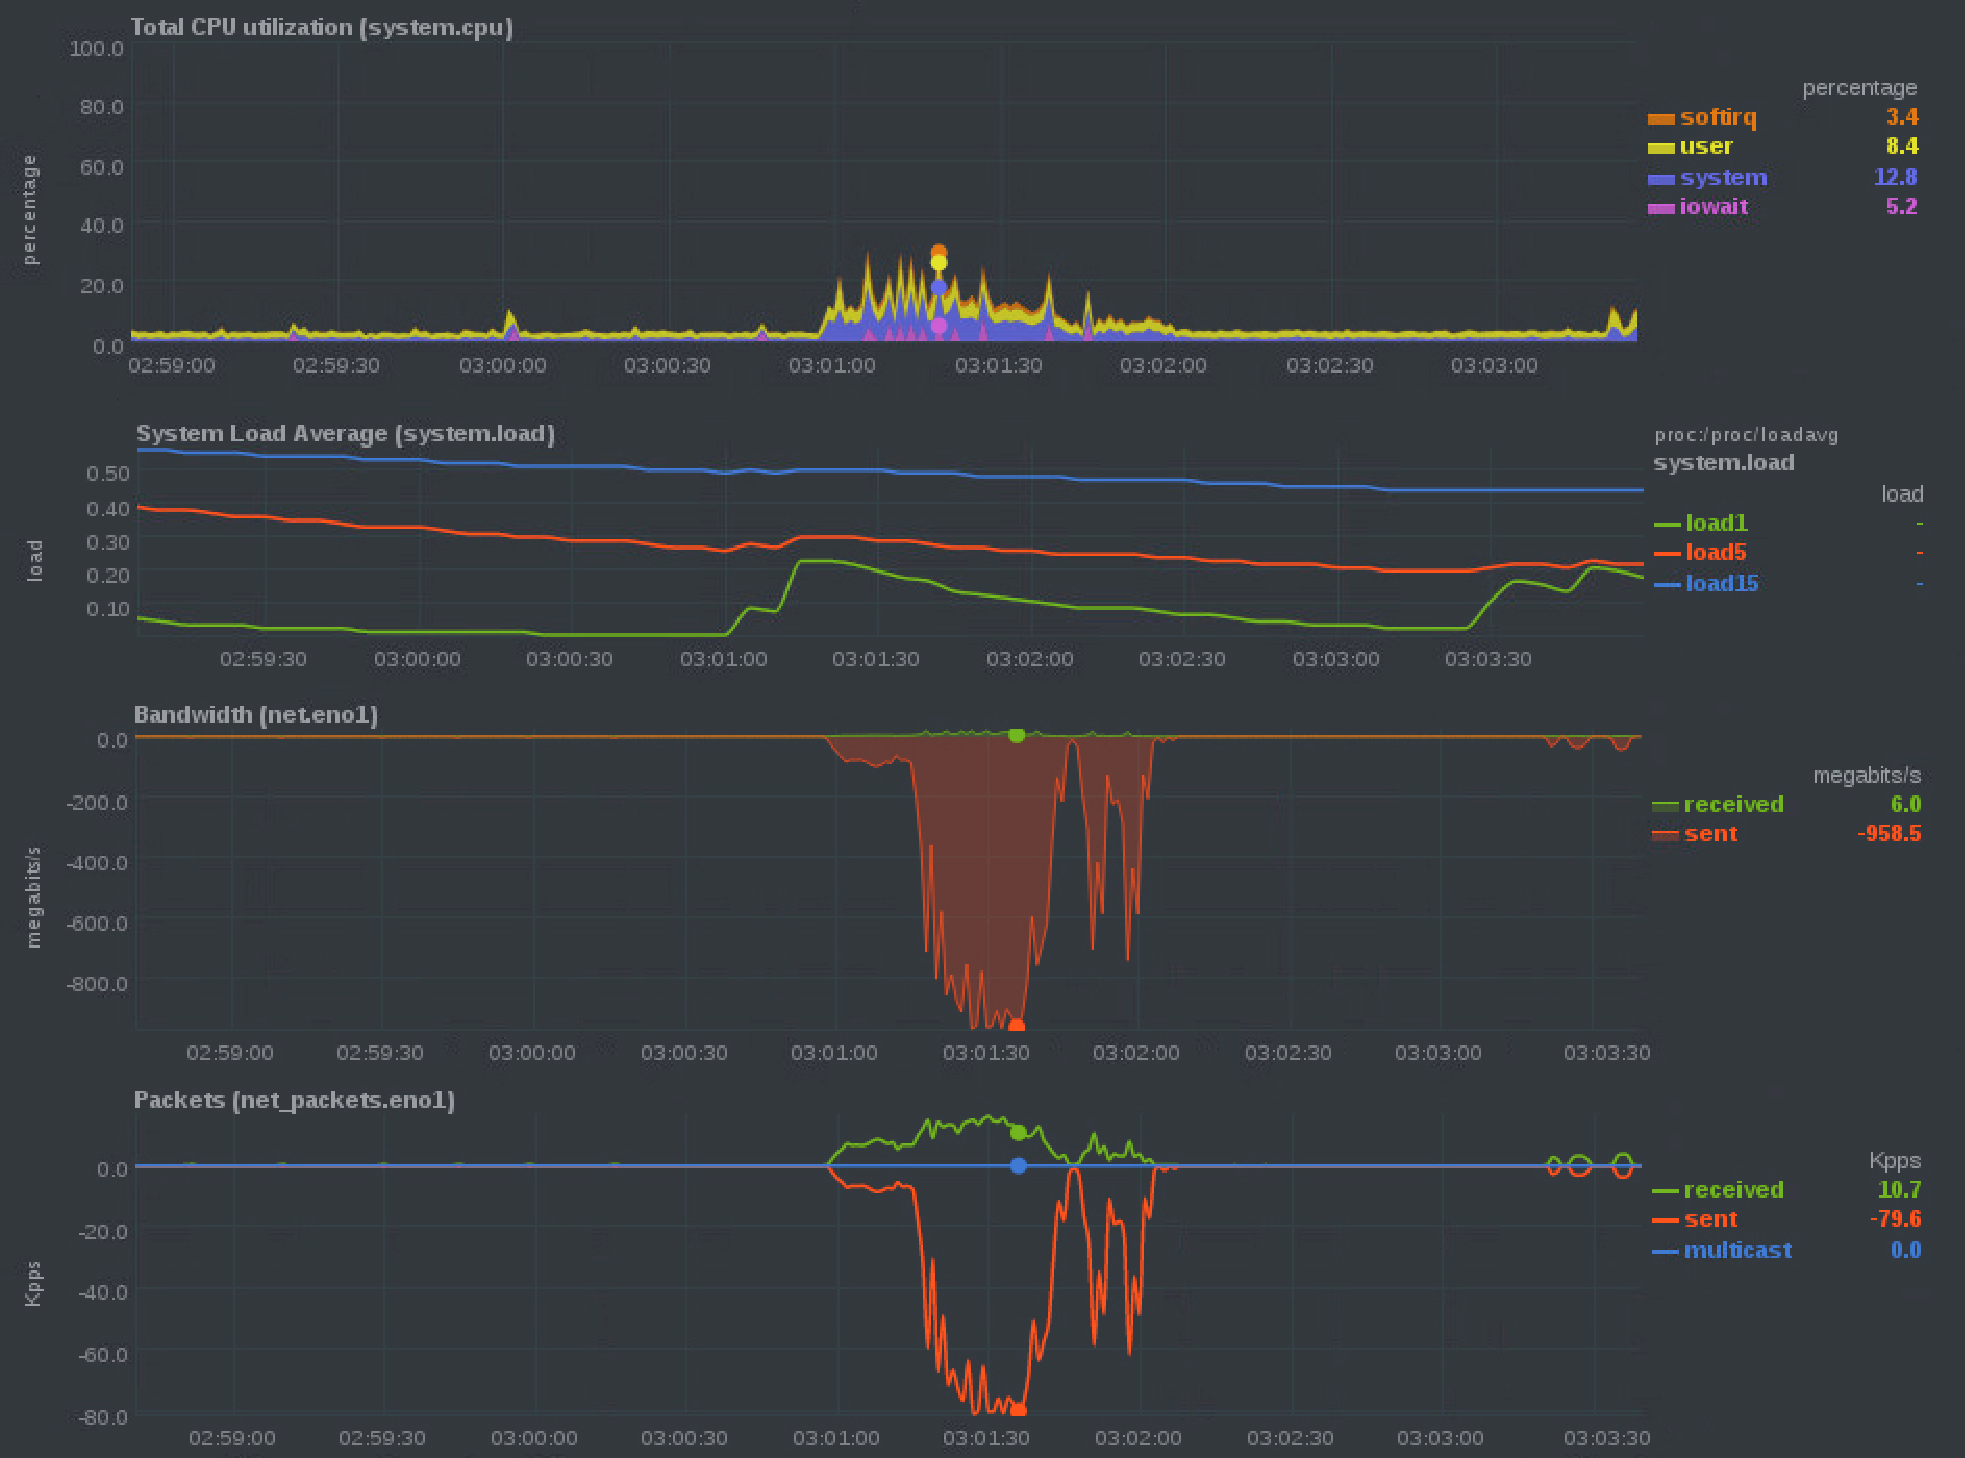
\includegraphics[height=4in]{cap5_bootstorm_cache_stats}
	\caption{System metrics for one run on the iCBD-Cache02 in a boot storm scenario}
	\label{fig:bootstorm_cache_stats}
\end{figure}



\begin{figure}[htbp]
	\centering
	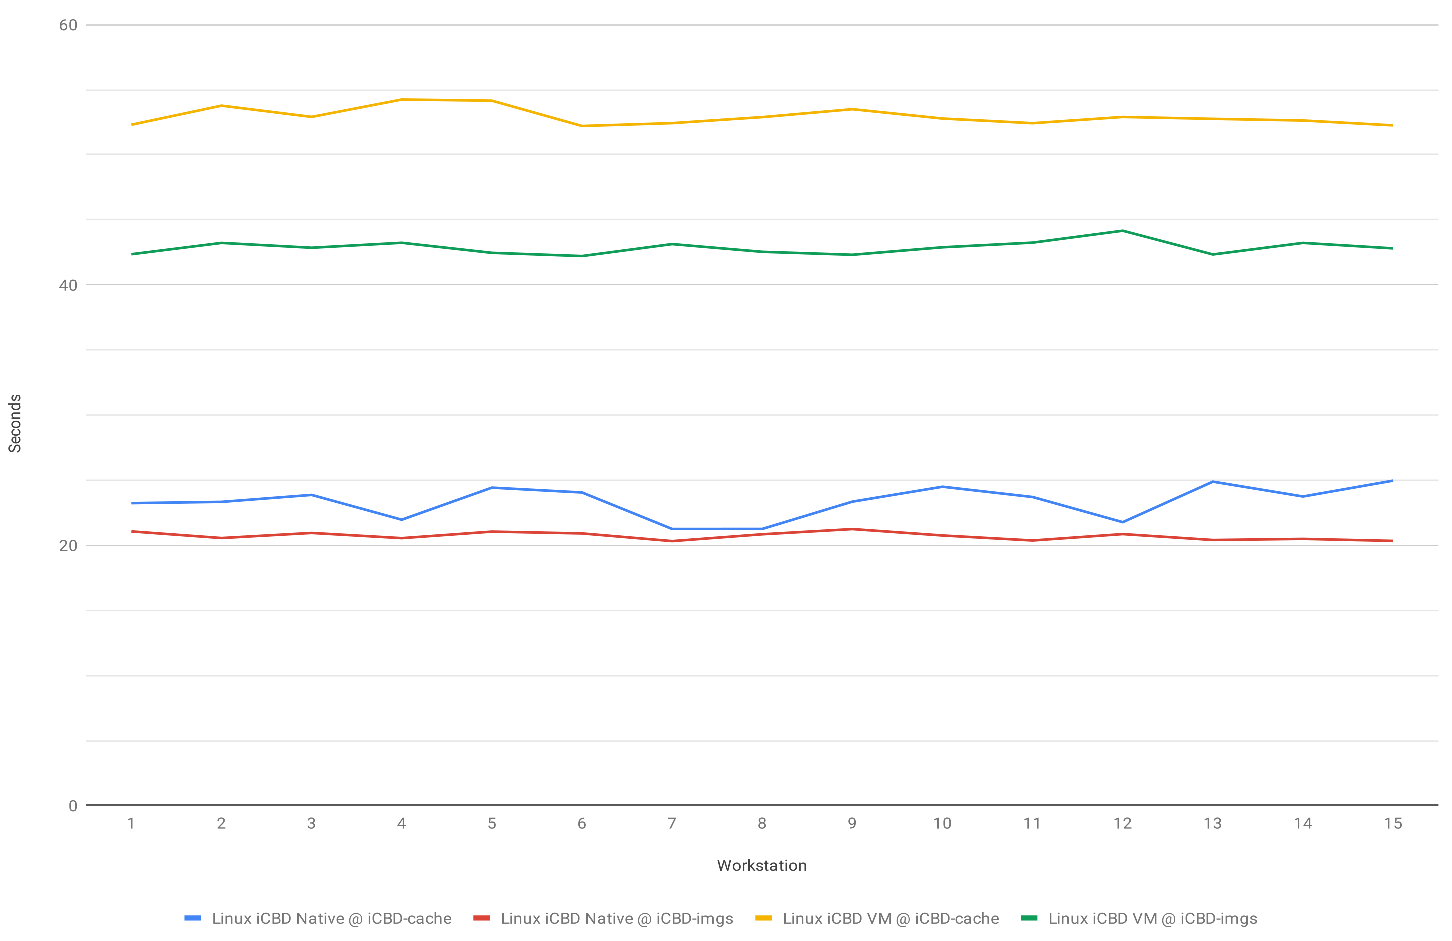
\includegraphics[height=4in]{cap5_BS_combo}
	\caption{Boot Time of fifteen workstations simultaneously (Boot Storm Scenario) comparing iMI provider using iSCSI}
	\label{fig:bootstorm_time}
\end{figure}



%\textbf{TOPICS :}
%\begin{itemize}
%	\item benchmarking 
%	\item Boot time Lab PC
%	\item Boot time iCBD VM in Cluster
%	\item Boot time iCBD in Lab PC (100 / 1000 mbps) iCBD-Imgs VM
%	\item Boot time iCBD in Lab PC (100 / 1000 mbps) iCBD-Cache
%\end{itemize}